The implementation follows these steps:
\begin{enumerate}
    \item \textbf{Image Preprocessing:} 
    \begin{itemize}
        \item Load the input image.
        \item Convert it to grayscale if necessary.
    \end{itemize}
    \item \textbf{Applying Otsu’s Thresholding:}
    \begin{itemize}
        \item Compute the optimal threshold automatically using Otsu’s method.
        \item Apply the threshold to generate a binary image.
    \end{itemize}
    \item \textbf{Visualization and Output:}
    \begin{itemize}
        \item Display both the original and thresholded images.
        \item Save the resulting binary image.
    \end{itemize}
\end{enumerate}

The function \texttt{otsu\_thresholding()} converts the image to grayscale if it is not already and then applies Otsu’s thresholding using \texttt{cv2.threshold()}. \\
The key component of the function is:
\begin{verbatim}
    _, binary_image = cv2.threshold(gray_image, 0, 255, cv2.THRESH_BINARY +
    cv2.THRESH_OTSU)
\end{verbatim}

Here, Otsu’s method automatically determines the threshold value by analyzing the image’s histogram and maximizing the inter-class variance. \\
Applying Otsu’s method to "houses.pgm" effectively separates the objects in the image from the background. The resulting binary image highlights structural details such as edges of buildings and other prominent objects.
\begin{figure}[H]
    \centering
    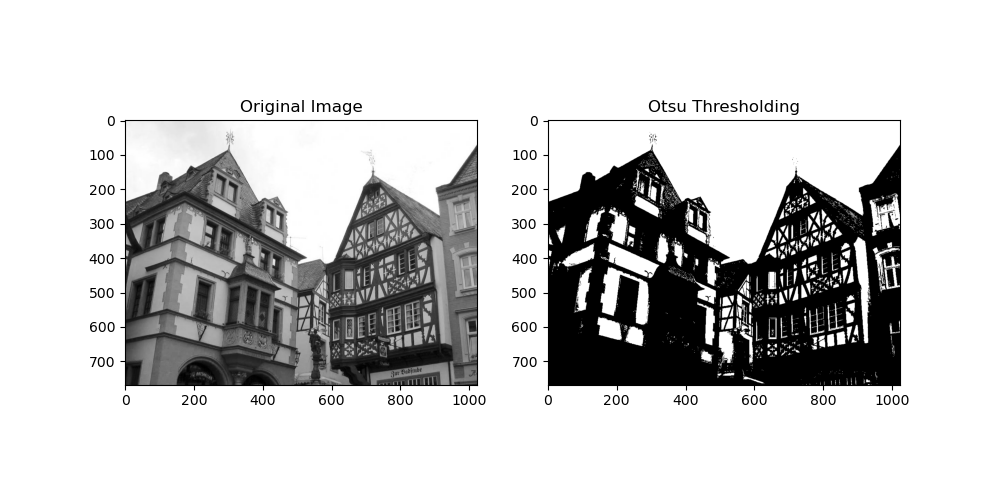
\includegraphics[width=\linewidth]{../Images/otsu_thresholding.png}
    \caption{Otsu method.}
    \label{fig:enter-label}
\end{figure}

The implementation successfully applies Otsu’s method to "houses.pgm," demonstrating its ability to segment objects efficiently.
\begin{figure}[H]
    \centering
    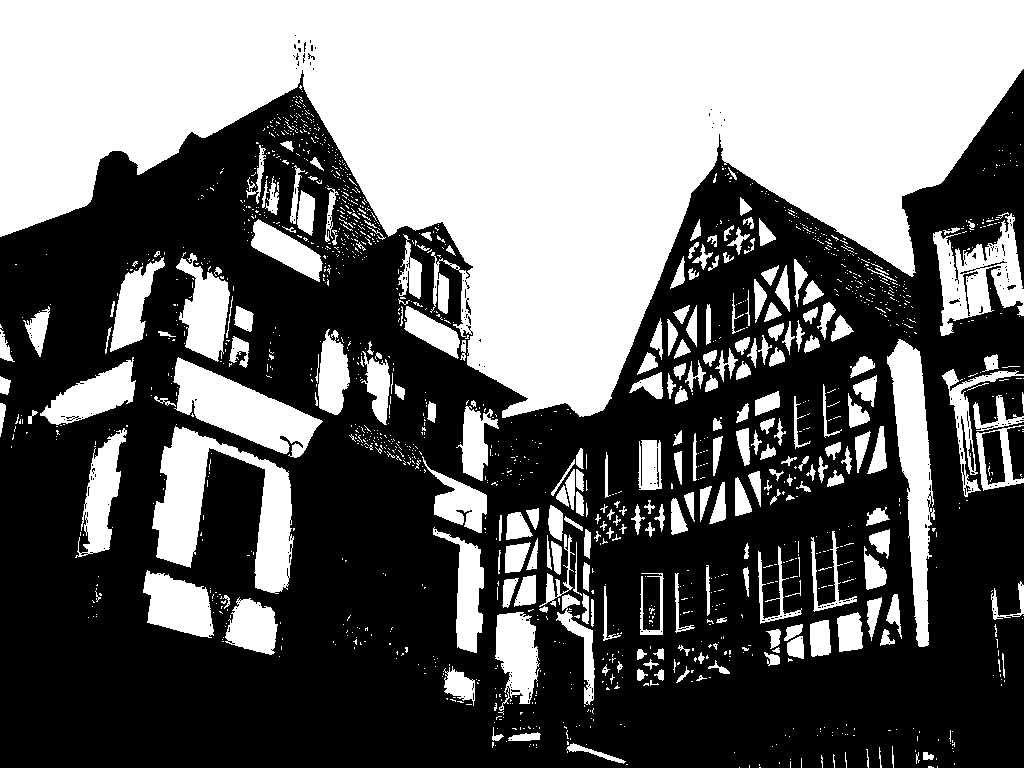
\includegraphics[width=0.65\linewidth]{../Images/binary_image.png}
    \caption{Final image.}
    \label{fig:enter-label}
\end{figure}
Future improvements could involve adaptive thresholding techniques for cases where global thresholding is insufficient due to uneven lighting conditions.